\documentclass{standalone}
\usepackage{tikz}

\definecolor{mBlue}{HTML}{22a1dc}
\definecolor{sBlue}{HTML}{009FE3}
\definecolor{sYellow}{HTML}{FFED00}
\definecolor{sRed}{HTML}{E30613}
\definecolor{sGreen}{HTML}{009640}
\definecolor{sPurple}{HTML}{440099}
\definecolor{mGreen}{HTML}{86cd30}
\definecolor{darkgreen}{HTML}{006400}
\definecolor{mLightBrown}{HTML}{e68a00}
\definecolor{lightred}{HTML}{FF9999}

%% COLOUR COMMANDS
\newcommand{\sBlue}[1]{\textcolor{sBlue}{#1}}
\newcommand{\sB}[1]{\sBlue{#1}}
\newcommand{\sRed}[1]{\textcolor{sRed}{#1}}
\newcommand{\sR}[1]{\sRed{#1}}
\newcommand{\sGreen}[1]{\textcolor{sGreen}{#1}}
\newcommand{\sG}[1]{\sGreen{#1}}
\newcommand{\sPurple}[1]{\textcolor{Purple}{#1}}
\newcommand{\sP}[1]{\sPurple{#1}}
\newcommand{\sYellow}[1]{\textcolor{sYellow}{#1}}
\newcommand{\sY}[1]{\sYellow{#1}}

\begin{document}
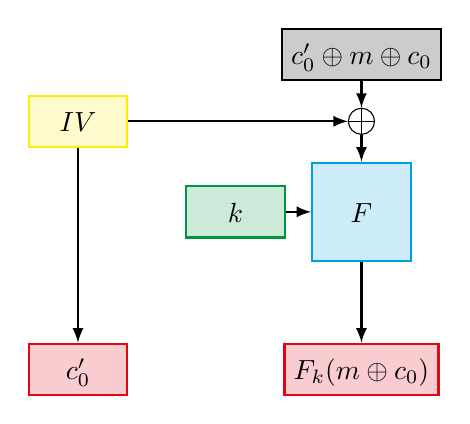
\begin{tikzpicture}[yscale=-1,xscale=0.8,>=latex]
		\tikzstyle{RECT} = [thick, minimum width=1.25cm, minimum height=0.65cm, text height=2ex, text depth=0.25ex]
		\tikzstyle{SQUA} = [thick, minimum width=1.25cm, minimum height =1.25cm, text height=2ex, text depth=0.25ex]
		\tikzstyle{key} = [RECT, draw=sGreen, fill=sGreen!20]
		\tikzstyle{prf} = [SQUA, draw=sBlue, fill=sBlue!20]
		\tikzstyle{tag} = [RECT, draw=sRed, fill=sRed!20]
		\tikzstyle{message} = [RECT, draw=black, fill=black!20]
		\tikzstyle{iv} = [RECT, draw=sYellow, fill=sYellow!20]
		\tikzset{XOR/.style={draw,circle,append after command={
					[shorten >=\pgflinewidth, shorten <=\pgflinewidth,]
					(\tikzlastnode.north) edge (\tikzlastnode.south)
					(\tikzlastnode.east) edge (\tikzlastnode.west)
				}
			}
		}
		

		\node[message] (mOne) at  	(0,  0) {$c_0' \oplus m \oplus c_0$};
		\node[XOR] (xOne) at 		(0, 0.85) {};
		\node[iv] (iOne) at 		(-4.5, 0.85) {$IV$};
		\node[key] (kOne) at 		(-2, 2) {$k$};
		\node[prf] (pOne) at		(0, 2) {$F$};
		\node[tag] (cOne) at		(0, 4) {$F_k(m \oplus c_0)$};
		\node[tag] (cZer) at		(-4.5,4) {$c_0'$};
		\draw[->, thick] (mOne.south) -- (xOne.north);
		\draw[->, thick] (xOne.south) -- (pOne.north);
		\draw[->, thick] (iOne.east) -- (xOne.west);
		\draw[->, thick] (kOne.east) -- (pOne.west);
		\draw[->,thick] (pOne.south) -- (cOne.north); 
		\draw[->,thick] (iOne.south) -- (cZer.north);
\end{tikzpicture}
\end{document}
